% Chapter 1
\chapter{Underlay Network}
\section{OpenvSwitch architecture}

When a packet first arrives to the switch it is sent straight to the controller to take the decisions of what to do with the packet if dropping the packet or setting a new flow entry for forwarding future similar packets.\\

The OpenVSwitch design is divided in two parts the kernel module and the userspace.
The kernel module follows the instructions and allocate some cached results.\\

In the userspace the ovs-switch matches the packets and openflow tables and then it sends this information to the controller to be stored in the ovsdb-server,  \autoref{fig:ovs} shows the process for the first packets and the different path for consecutive packets, with an example of sending them to Virtual machines.\\


\begin{figure}[bth]
{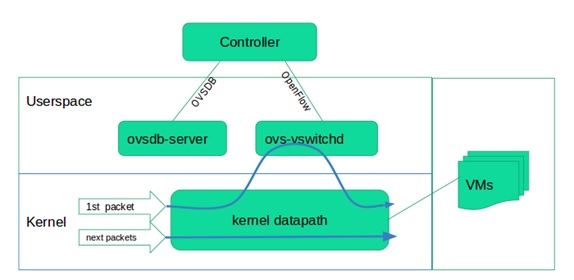
\includegraphics[width=1.2\linewidth]{gfx/ovs}}\caption[OpenvSwitch Architecture]{OpenvSwitch Architecture}
{\label{fig:ovs}
\end{figure}

\section{Containers} 

Container shares the same kernel having less weight.\\

Containers are processes that are isolated from the rest of the machine, it can encapsulate any application dependencies, multiple applications can coexist in the same environment, it also speedup the application development by building the application only once and being able to run in every kind of environment.\\

Main characteristics applied to the model\\

Docker containers add a new layer of virtualization to the environment one physical device can have many virtual machines and on each virtual machine there can be many containers; for the containers to communicate with Virtual machines and within other containers, the inter-connection is not as straightforward as traditional topologies.\\

Since docker containers can access the kernel, docker provide a feature that will control the restrictions of the view of the system, namespaces are the ones that verify whether a user is allowed to access a specific file, process, etc.\\

To get an insight of the network infrastructure of docker containers, I used The commands used for this are in the paper of Virtualization-A highlight on performance \cite{3} written by my previous tutor Guillaume Urvoy-Keller, and docker tutorials\cite{4}. I used all the information and summarized it in the next steps which are important for the development of this project.\\

\section{Practical experimentation and issues}

This project was developed in a PC with 8,00GB of RAM and a quad-core processor, I installed Ubuntu on a dual boot and on the top of the Ubuntu Operating system I installed Docker infrastructure.\\

First it is important to know that docker containers create by default a docker0 network that at the moment a container start running it creates a veth peer link to the docker0 network and create a new network namespace in the container. To  eliminate this docker0 network while running a new container we can specify that we don’t want any network description to be attached to our running container with the flag –net=’none’   or we can  bring docker0 down.\\

This will help in the future to avoid problems at the moment of appending to the underlying network and for migration of containers.\\
\begin{itemize}
\item Creation of a New container:\\
\texttt{docker run --name=controller --net='none' -ti ubuntu /bin/bash}\\
\item Two containers linked with the use of namespace:\\
This information is important since in the installation of the services of Open Stack we can see a similar approach, they use the same way of configuring different nodes for stating which service is going to be the controller.\\
\texttt{docker run -ti --name compute --link controller:controller ubuntu /bin/bash}\\
This command links a container that was previously created (controller) with a new container created called compute, but it is only a one way connection, so for the compute node I created  the \texttt{/etc/hosts} file as well.
\item Two containers with OpenvSwitch:\\
\texttt{ovs-vsctl add-br s1}\\
\texttt{ifconfig br1 192.168.0.1 netmask 255.255.255.0}

\end{itemize}

Since docker containers have assigned each a unique namespace we have to create also the network namespace, for doing this we need to check the process id of the container that we are planning to join to my network and store its value in the file \texttt{/var/run/netns}\\

To learn the process id of the controller:\\
\texttt{docker inspect -f '{{.State.Pid}}' <process id of c1>}\\
After this we get the process id and we create a namespace entry in \texttt{/var/run/netns} to specify the connection.\\

\texttt{pid=} #here we have to write the new process id\\
\texttt{mkdir -p /var/run/netns}\\
\texttt{ln -s /proc/$pid/ns/net /var/run/netns/$pid}\\

Note: to check the process id: \texttt{docker ps}\\
 
Next it was created a peer of interfaces c1-eth0 corresponding to the network namespace of the container c1 and s1-eth1 corresponding to the OpenvSwitch s1 that was previously created; next it was assigned an ip and a default route \autoref{fig:dockerconnected}, shows this architecture.\\

\begin{figure}[bth]
{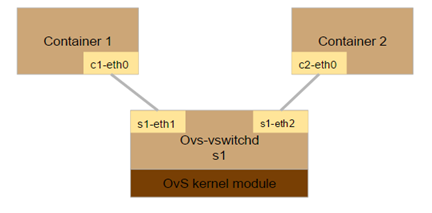
\includegraphics[width=1.2\linewidth]{gfx/dockerconnected}}\caption[OpenvSwitch connected with 2 docker containers]{OpenvSwitch connected with 2 docker containers}
{\label{fig:dockerconnected}
\end{figure}


For the creation of the peer interfaces c1-eth0 and s1-eth1, and for binding s1-eth1 to the bridge s1 I did the next:\\

\texttt{ip link add c1-eth0 type veth peer name s1-eth1}\\
\texttt{ovs-vsctl add-port s1 s1-eth1}\\
\texttt{ip link set s1-eth1 up}\\

Next to bind c1-eth0 to the container network namespace assigning an ip\\

\begin{lstlisting}[language=bash,frame=tb,caption={Network namespaces creation}]
ip link set c1-eth0 netns $pid
ip netns exec $pid ip link set c1-eth0 address 12:34:56:78:9a:bc
ip netns exec $pid ip link set c1-eth0 up
ip netns exec $pid ip addr add 192.168.0.0/24 dev c1-eth0
ip netns exec $pid ip route add default via 192.168.0.1
\end{lstlisting}\\

All this experimentations provide many different ways for containers to be inter-connected between each other, attaching containers together, using linux bridges or docker containers, but since in the next part of the work I will be using Multi-host configuration and I will need to configure OpenStack Self Services, I tried it with OpenVSwitch and Linux Bridge to choose the best in performance.\\

To choose the right approach I have tested different situations and architectures.
I used docker containers since they are more lightweight than hypervisors they can run up to 10.000 of containers in one host, containers use cgroups and namespaces.\\

\section{Analysis}
\subsection{Linux bridge vs OpenvSwitch}\\

When we run a new container or when several containers run they by default a create a linux bridge for connectivity between containers, the problem with linux bridges is that it has a limit in scalability since it only has 1024, since Docker containers and Openstack Virtual machines are in a different level of virutalization the best aproach is to use OpenvSwitch.\\

\subsubsection{Benchmarking}

Cpu Benchmarking:\\

First I had use Docker containers and Vagrant virtual machines and with the use of sysbench with  1000 of computations for computing prime numbers with 2 CPUs available give to a result that the time average to perform the computation on a docker container was almost half quick as the time on Vagrant virtual machines.\\

Network Benchmarking \\

For the network benchmarking I run two nodes one as a client \texttt{iperf -c} and the other as a server \texttt{iperf -s} and transferring messages with the results shown in the next chart we can see that Docker with OVS is a faster approach.\\

Ipef is used to check the network bandwith and the quality of the link.\\

\autoref{fig:benchmark} presents the throughput of the iperf command by sending messages from 64MB with the -m option and so on decreasing the bandwith 

\begin{figure}[bth]
{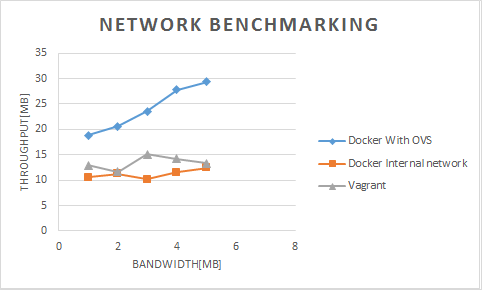
\includegraphics[width=1.2\linewidth]{gfx/benchmark}}\caption[Throughput: performance after iperf command]{Throughput: performance after iperf command}
{\label{fig:benchmark}
\end{figure}\\

The partial conclusion of this part of the project explains why I chose to use a Docker container with OpenvSwitch since as shown in the figure above this architecture has a more efficient support. 

\marginpar{Docker with ovs provide a better throughput specially for smaller bandwidth}
\\

\subsection{Docker with OpenStack}

Docker containers can run any kind of software they are configured to run, to learn how to configure each container it is important to know the different functions that docker can offer, the docker engine provides fast to test and deploy applications.\\

To develop the configuration of this applications docker engine uses dockerfile. Docker file contains the configuration that the service needs, it has linux command and docker commands for installation of packages.\\

For the configuration of the container to be saved, it is needed to commit the changes and save them, we can also save them in a repository, Docker has a SaaS service for sharing a repository called Dockerhub.\cite{4}\\

In this part of the project I pulled a container from the repository continues/openstack-controller, continues/openstack-network, continues/openstack-compute that has the basic configuration of OpenStack, and added the respective configuration provided by OpenStack self-services in the next section there is the explanation of the motive to choose OpenStack Self Services.\\

Example of dockerfile:\\
\begin{lstlisting}[language=yaml,frame=tb,caption={Dockerfile}]
FROM ubuntu:14.04
RUN apt-get update \
	&& apt-get -y install software-properties-common python-software-properties \
	&& add-apt-repository -y cloud-archive:mitaka \
	&& apt-get update \
	&& apt-get -y dist-upgrade \
	&& apt-get -y install python-mysqldb 
RUN apt-get -y install neutron-plugin-ml2 neutron-plugin-openvswitch-agent \
    neutron-l3-agent neutron-dhcp-agent
EXPOSE 9696
\end{lstlisting}\\

Note: To save the containers configuration\\
\texttt{Docker commit <process id> anabeldlw/openstack<service>:<version>}\\

After commiting the configuration of the container we need to tag and push them to the repository.\\

First we learn the image id with the docker images command, then we need to copy the id for the name of the image as shown in the next example:\\
\begin{lstlisting}[language=yaml,frame=tb,caption={Dockerfile}]
$docker images
REPOSITORY				       TAG	 IMAGE ID	   CREATED 	    SIZE
anabeldlw/openstack_controller	tag1 71c0daa71ae8 3 days ago 	718MB

$docker tag 71c0daa71ae8 anabeldlw/openstack_controller:tag1
$docker push anabeldlw/openstack_controller:tag1
\end{lstlisting}\\

Network configuration on OpenStack:

In this section there will be an explanation of the Self-service networks and the provider networks and why did I choose to use the Self-service networks.
Provider networks:
It is managed only by administrators, since they need the configuration of a physical network infrastructure. This networks only handle layer 2 connectivity for instances
Self-service networks: 
The advantage of the self-service networks over the provider network is that with self-services it is possible to enable projects to manage networks totally virtual, without involving administrators.
The support of networks without overlapping IP addresses will be done by the use of the VXLAN and GRE protocols, in contrast to the provider networks that are using layer 2 segmentation.https://docs.openstack.org/mitaka/networking-guide/deploy-ovs-selfservice.html
IPv4 usually use private IP addresses according to RFC7348 https://tools.ietf.org/html/rfc7348 with NAT and floating IP addresses on virtual routers to enable access from provider networks while IPv6 uses public IP addresses with static routes. 
This network service use Layer 3 routers that reside in a network node in contrary to provider networks that rely in physical network. 
After reviewing this descriptions for the network configuration of OpenStack I reached to the conclusion that for the network configuration of OpenStack to work in concordance with the one of docker containers, need to be the one fully virtualized, network self services.
The requirements for the Self-service network are the next:
In the controller node: 
-2 network interfaces (management and provider)
-sql service with  databases for OpenStack
-keystone, glance, nova 
-neutron and ML2 plugin
In the network node:
-layer 3 (routing component) and dependencies
-3 network interfaces(management, provider and overlay)
-Layer 2 agent
Compute node: 
-hypervisor(nova)
-layer 2, DHCP, metadata
-2 network interfaces (management, provider)

For the configuration of the VXLAN in the controller node, the VNI has to be chosen and as specified in the RFC7348 document https://tools.ietf.org/html/rfc7348 
“The VNI is in an outer header that encapsulates the inner MAC frame originated by the VM”. 
This document explain how the VNI is used for the encapsulation of inner MAC addresses produced by virtual machine addresses so if there is an overlapping of physical and virtual machine addresses, the VNI will identify the inner virtual machine addresses.



\texttt{Elasticsearch}  has 2 type of nodes the data nodes and non data nodes.
\\

The \textbf{data nodes} hold and perform data related operations and the \textbf{non data nodes} are divided in three different node types:
\begin{itemize}
\item The \texttt{master node}, that controls the cluster and can behave as a coordinating node
\item The \texttt{client nodes} that can neither hold data nor become the master node, it behaves as a smart router.
\item the {tribe node} which can connect to different clusters.
\end{itemize}
\subsubsection{Searching in different nodes}
\paragraph{Scatter Phase} Each data node executes the request locally
\paragraph{Gather Phase} Manage the requests to the data nodes holding the data\\

It is important to split the data from non data to data nodes, since indexing and searching can put a lot of pressure in the nodes resource. 
\\

It is very important that the master eligible nodes do as little work as possible since master nodes can behave as a coordinating nodes.

\subsubsection{Split brain prevention}
The minimum number of master eligible nodes in order to join a cluster must be 2 and the most appropriate at the moment of building an infrastructure follows the next equation:

\begin{equation}
(master\_elegible\_nodes / 2)+1
\end{equation}
In order to explain this, lets suppose a case when there are 3 nodes in the cluster and there is a network failure.
\begin{itemize}
\item In the \texttt{First case} if there is only a master eligible node as soon as the two parts of the cluster are not communicating each other they cannot find the master eligible node and choose themselves as a master creating a split brain, and when rejoining the cluster one of this master eligible nodes will have to be restarted loosing all its information.
\item In the \texttt{Second case} if the minimum master nodes is 2, one of the nodes wont see another master eligible node so it wont be able to choose itself as a master node, when the communication is restored it can rejoin the cluster and work normally 
\end{itemize}

\subsection{Logstash}

Logstash is used to collect, organize and processes all kind of data, its plugable architecture is very simple, it contains filters, inputs and outputs, it uses regular expressions which facilitate the methods of aggregating and grouping data.

\paragraph{input} It is used for collecting data from different sources, adding the path or plugin from which the data will be retreived, \eg event logs, data stored in elasticsearch, etc.
\paragraph{filter} To organize the data collected and to retreive only the fields needed, Logstash configuration has the possibility of adding filters, depending on the characteristics of the documents parsed, filters as \texttt{grok}, to search with the use of regular expresions over the document or \texttt{mutate} to omit the extraction of some fields or part of the documents. 
\\

Grok works by parsing text patterns, using regular expressions, and assigning them to an identifier.
\\

The syntax for a grok pattern is \%\{PATTERN:IDENTIFIER\}. A Logstash filter includes a sequence of grok patterns that matches and assigns various pieces of a log message to various identifiers, which is how the logs are given structure\cite{1}.

\paragraph{output} To send the processed data to the servers for a furhter vizualization and analysis.

\subsection{Kibana}

Kibana is used for the vizualization and interaction with data filtered and stored in elasticsearch, it offers a web interface to search visualize and create dashboards for the overview of the usefull contents.
\\

Kibana offers the next visualization types:
\begin{itemize}
\item Area Chart
\item Data table
\item Line Chart
\item Markdown widget
\item Metric
\item Pie chart
\item Title map
\item Vertical bar chart
\end{itemize}

One of the most usefull features of kibana is the aggregation builder for choosing the count, average, min, sum, max or cardinality, with this the metrics of the y or x axis can be changed sorting by different terms.
\\

There is a part very important to take into account in kibana since the extracting of data is made by word each field that is separated by a space is called an Analized fields. 
\\

Analized fields can trouble the search since instead of grouping by one single word, it sort by two words as if they where separated fields providing a bad information of the analysis of the data, meaning that if a specific word that represent only to one field but has a space will be discplayed as two different words and the analytics will display the information twice instead of only ones
\\

To avoid porblems with this it is very usefull to change this analyzed fields to not analyzed in the configuration files before indexing, since this fields cannot be changed after they had been pushed to elasticsearch.
